\XtoCBlock{Sin2Limiter}
\label{block:Sin2Limiter}
\begin{figure}[H]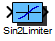
\includegraphics{Sin2Limiter}\end{figure} 

\begin{XtoCtabular}{Inports}
In & \tabularnewline
\hline
\end{XtoCtabular}


\begin{XtoCtabular}{Outports}
Out & \tabularnewline
\hline
\end{XtoCtabular}

\begin{XtoCtabular}{Mask Parameters}
Tr & Rising time in seconds. Slew rate will be 1/Tr\tabularnewline
\hline
Tf & Falling time in seconds. Slew rate will be 1/Tf\tabularnewline
\hline
ts\_fact & Multiplication factor of base sampling time (in integer format)\tabularnewline
\hline
\end{XtoCtabular}

\subsubsection*{Description:}
Limitation of rising and falling rate with sin\textasciicircum{}2 characteristic.

    Note: A running limitation process can not be interrupted!

% include optional documentation file
\InputIfFileExists{\XcHomePath/Library/General/Doc/Sin2Limiter_Info.tex}{\vspace{1ex}}{}

\subsubsection*{Implementations:}
\begin{tabular}{l l}
\textbf{FiP8} & 8 Bit Fixed Point Implementation\tabularnewline
\textbf{FiP16} & 16 Bit Fixed Point Implementation\tabularnewline
\textbf{FiP32} & 32 Bit Fixed Point Implementation\tabularnewline
\textbf{Float32} & 32 Bit Floating Point Implementation\tabularnewline
\textbf{Float64} & 64 Bit Floating Point Implementation\tabularnewline
\end{tabular}

\XtoCImplementation{FiP8}
\index{Block ID!112}
\nopagebreak[0]
% Implementation details
\begin{tabular}{l l}
\textbf{Name} & FiP8 \tabularnewline
\textbf{ID} & 112 \tabularnewline
\textbf{Revision} & 0.2 \tabularnewline
\textbf{C filename} & Sin2Limiter\_FiP8.c \tabularnewline
\textbf{H filename} & Sin2Limiter\_FiP8.h \tabularnewline
\end{tabular}
\vspace{1ex}

8 Bit Fixed Point Implementation

\begin{XtoCtabular}{Controller Parameters}
RateUp & Rising time parameter\tabularnewline
\hline
RateDown & Falling time parameter\tabularnewline
\hline
Scaled\_RateUp & To step height scaled rising time parameter\tabularnewline
\hline
Scaled\_RateDown & To step height scaled falling time parameter\tabularnewline
\hline
Out\_end & Desired target value\tabularnewline
\hline
Level & Current level of internal ramp from 1 to 0\tabularnewline
\hline
Step\_Height & Active step height\tabularnewline
\hline
State & Current state of limitation\tabularnewline
\hline
\end{XtoCtabular}

% Implementation data structure
\XtoCDataStruct{Data Structure:}
\begin{lstlisting}
typedef struct {
     uint16        ID;
     int8          *In;
     int8          Out;
     int16         RateUp;
     int16         RateDown;
     int16         Scaled_RateUp;
     int16         Scaled_RateDown;
     int8          Out_end;
     uint16        Level;
     int16         Step_Height;
     int8          State;
} SIN2LIMITER_FIP8;
\end{lstlisting}

\ifdefined \AddTestReports
\InputIfFileExists{\XcHomePath/Library/General/Doc/Test_Sin2Limiter_FiP8.tex}{}{}
\fi
\XtoCImplementation{FiP16}
\index{Block ID!113}
\nopagebreak[0]
% Implementation details
\begin{tabular}{l l}
\textbf{Name} & FiP16 \tabularnewline
\textbf{ID} & 113 \tabularnewline
\textbf{Revision} & 0.2 \tabularnewline
\textbf{C filename} & Sin2Limiter\_FiP16.c \tabularnewline
\textbf{H filename} & Sin2Limiter\_FiP16.h \tabularnewline
\end{tabular}
\vspace{1ex}

16 Bit Fixed Point Implementation

\begin{XtoCtabular}{Controller Parameters}
RateUp & Rising time parameter\tabularnewline
\hline
RateDown & Falling time parameter\tabularnewline
\hline
Scaled\_RateUp & To step height scaled rising time parameter\tabularnewline
\hline
Scaled\_RateDown & To step height scaled rising time parameter\tabularnewline
\hline
Out\_end & Desired target value\tabularnewline
\hline
Level & Current level of internal ramp from 1 to 0\tabularnewline
\hline
Step\_Height & Active step height\tabularnewline
\hline
State & Current state of limitation\tabularnewline
\hline
\end{XtoCtabular}

% Implementation data structure
\XtoCDataStruct{Data Structure:}
\begin{lstlisting}
typedef struct {
     uint16        ID;
     int16         *In;
     int16         Out;
     int32         RateUp;
     int32         RateDown;
     int32         Scaled_RateUp;
     int32         Scaled_RateDown;
     int16         Out_end;
     uint32        Level;
     int32         Step_Height;
     int8          State;
} SIN2LIMITER_FIP16;
\end{lstlisting}

\ifdefined \AddTestReports
\InputIfFileExists{\XcHomePath/Library/General/Doc/Test_Sin2Limiter_FiP16.tex}{}{}
\fi
\XtoCImplementation{FiP32}
\index{Block ID!114}
\nopagebreak[0]
% Implementation details
\begin{tabular}{l l}
\textbf{Name} & FiP32 \tabularnewline
\textbf{ID} & 114 \tabularnewline
\textbf{Revision} & 0.2 \tabularnewline
\textbf{C filename} & Sin2Limiter\_FiP32.c \tabularnewline
\textbf{H filename} & Sin2Limiter\_FiP32.h \tabularnewline
\end{tabular}
\vspace{1ex}

32 Bit Fixed Point Implementation

\begin{XtoCtabular}{Controller Parameters}
RateUp & Rising time parameter\tabularnewline
\hline
RateDown & Falling time parameter\tabularnewline
\hline
Scaled\_RateUp & To step height scaled rising time parameter\tabularnewline
\hline
Scaled\_RateDown & To step height scaled rising time parameter\tabularnewline
\hline
Out\_end & Desired target value\tabularnewline
\hline
Level & Current level of internal ramp from 1 to 0\tabularnewline
\hline
Step\_Height & Active step height\tabularnewline
\hline
State & Current state of limitation\tabularnewline
\hline
\end{XtoCtabular}

% Implementation data structure
\XtoCDataStruct{Data Structure:}
\begin{lstlisting}
typedef struct {
     uint16        ID;
     int32         *In;
     int32         Out;
     int32         RateUp;
     int32         RateDown;
     int32         Scaled_RateUp;
     int32         Scaled_RateDown;
     int32         Out_end;
     uint32        Level;
     int32         Step_Height;
     int8          State;
} SIN2LIMITER_FIP32;
\end{lstlisting}

\ifdefined \AddTestReports
\InputIfFileExists{\XcHomePath/Library/General/Doc/Test_Sin2Limiter_FiP32.tex}{}{}
\fi
\XtoCImplementation{Float32}
\index{Block ID!115}
\nopagebreak[0]
% Implementation details
\begin{tabular}{l l}
\textbf{Name} & Float32 \tabularnewline
\textbf{ID} & 115 \tabularnewline
\textbf{Revision} & 0.1 \tabularnewline
\textbf{C filename} & Sin2Limiter\_Float32.c \tabularnewline
\textbf{H filename} & Sin2Limiter\_Float32.h \tabularnewline
\end{tabular}
\vspace{1ex}

32 Bit Floating Point Implementation

\begin{XtoCtabular}{Controller Parameters}
RateUp & Rising time parameter\tabularnewline
\hline
RateDown & Falling time parameter\tabularnewline
\hline
Scaled\_RateUp & To step height scaled rising time parameter\tabularnewline
\hline
Scaled\_RateDown & To step height scaled falling time parameter\tabularnewline
\hline
Out\_end & Desired target value\tabularnewline
\hline
Level & Current level of internal ramp from pi/2 to 0\tabularnewline
\hline
Step\_Height & Active step height\tabularnewline
\hline
State & Current state of limitation\tabularnewline
\hline
\end{XtoCtabular}

% Implementation data structure
\XtoCDataStruct{Data Structure:}
\begin{lstlisting}
typedef struct {
     uint16        ID;
     float32       *In;
     float32       Out;
     float32       RateUp;
     float32       RateDown;
     float32       Scaled_RateUp;
     float32       Scaled_RateDown;
     float32       Out_end;
     float32       Level;
     float32       Step_Height;
     int8          State;
} SIN2LIMITER_FLOAT32;
\end{lstlisting}

\ifdefined \AddTestReports
\InputIfFileExists{\XcHomePath/Library/General/Doc/Test_Sin2Limiter_Float32.tex}{}{}
\fi
\XtoCImplementation{Float64}
\index{Block ID!116}
\nopagebreak[0]
% Implementation details
\begin{tabular}{l l}
\textbf{Name} & Float64 \tabularnewline
\textbf{ID} & 116 \tabularnewline
\textbf{Revision} & 0.1 \tabularnewline
\textbf{C filename} & Sin2Limiter\_Float64.c \tabularnewline
\textbf{H filename} & Sin2Limiter\_Float64.h \tabularnewline
\end{tabular}
\vspace{1ex}

64 Bit Floating Point Implementation

\begin{XtoCtabular}{Controller Parameters}
RateUp & Rising time parameter\tabularnewline
\hline
RateDown & Falling time parameter\tabularnewline
\hline
Scaled\_RateUp & To step height scaled rising time parameter\tabularnewline
\hline
Scaled\_RateDown & To step height scaled falling time parameter\tabularnewline
\hline
Out\_end & Desired target value\tabularnewline
\hline
Level & Current level of internal ramp from pi/2 to 0\tabularnewline
\hline
Step\_Height & Active step height\tabularnewline
\hline
State & Current state of limitation\tabularnewline
\hline
\end{XtoCtabular}

% Implementation data structure
\XtoCDataStruct{Data Structure:}
\begin{lstlisting}
typedef struct {
     uint16        ID;
     float64       *In;
     float64       Out;
     float64       RateUp;
     float64       RateDown;
     float64       Scaled_RateUp;
     float64       Scaled_RateDown;
     float64       Out_end;
     float64       Level;
     float64       Step_Height;
     int8          State;
} SIN2LIMITER_FLOAT64;
\end{lstlisting}

\ifdefined \AddTestReports
\InputIfFileExists{\XcHomePath/Library/General/Doc/Test_Sin2Limiter_Float64.tex}{}{}
\fi
